\documentclass[12pt,a4paper,openright,twoside]{book}
\usepackage{acronym}
\usepackage[utf8]{inputenc}
\usepackage{disi-thesis}
\usepackage{code-lstlistings}
\usepackage{notes}
\usepackage{shortcuts}
\usepackage{empheq}

\school{\unibo}
\programme{Corso di Laurea Triennale in Ingegneria e Scienze Informatiche}
\title{Prototipo d'Irrigazione di Precisione}
\author{Davide Speziali}
\date{\today}
\subject{Supervisor's course name}
\supervisor{Prof. Supervisor Here}
\cosupervisor{Dott. CoSupervisor 1}
\morecosupervisor{Dott. CoSupervisor 2}
\session{I}
\academicyear{2023-2024}

% Definition of acronyms
\acrodef{IoT}{Internet of Thing}
\acrodef{GPIO}{General Purpose Input/Output}
\acrodef{PWM}{pulse-width modulation}
\acrodef{SBC}{Single Board Computer}
\acrodef{JS}{JavaScript}
\acrodef{ONU}{Organizzazione delle Nazioni Unite}
\acrodef{SDG}{Sustainable Development Goals}
\acrodef{FC}{Field Capacity}
\acrodef{PWP}{Permanent Wilting Point}
\acrodef{SWRC}{Soil Water Retention Curve}
\acrodef{SWC}{Soil Water Content}
\acrodef{SWP}{Soil Water Potential}
\acrodef{$ET_0$}{potential evapotranspiration}
\acrodef{$ET_a$}{actual evapotranspiration}
\acrodef{$K_c$}{crop coefficient}
\acrodef{GPS}{Global Positioning System}
\acrodef{SSLM}{Site-Specific Land Management}
\acrodef{SSNM}{Site-Specific Nutrient Management}
\acrodef{SSWM}{Site-Specific Weed Management}
\acrodef{SSCP}{Site Specific Crop Protection}
\acrodef{GIS}{Geographical Information System}
\acrodef{CSM}{Crop Simulation Model}
\acrodef{VRT}{Variable Rate Technology}
\acrodef{DSS}{Decision Support System}
\acrodef{PID}{proporzionale-integrale-derivativo}
\acrodef{LPWA}{Low-Power Wide-Area}
\acrodef{MPC}{Model Predictive Control}
\mainlinespacing{1.241} % line spacing in mainmatter, comment to default (1)

\begin{document}
\frontmatter\frontispiece
%
% \begin{abstract}
%     TODO
% \end{abstract}

% \begin{dedication} % this is optional
%     Optional. Max a few lines.
% \end{dedication}
%
%----------------------------------------------------------------------------------------
\tableofcontents
\listoffigures     % (optional) comment if empty
%\lstlistoflistings % (optional) comment if empty

\mainmatter
%
% \chapter*{Introduzione}
% \addcontentsline{toc}{chapter}{Introduzione}
% \setcounter{chapter}{0}
%
% \paragraph{Structure of the Thesis}
% \note{At the end, describe the structure of the paper}
\chapter{Agricultura di precisione}
%
La lotta al cambiamento climatico è uno dei temi più importanti per il futuro delle popolazioni del pianeta.
A partire dal 2015 l'\ac{ONU}, con l'obiettivo di rispondere in maniera sistematica al problema del cambiamento climatico, ha adottato l'Agenda 2030 per lo Sviluppo Sostenibile.
In questo contesto vengono specificate 16 \ac{SDG}: obiettivi comuni su questioni importanti per lo sviluppo tra cui la lotta alla povertà, l'eliminazione della fame e il contrasto al cambiamento climatico. Tra essi \ac{SDG} 6 "Acqua pulita e sanificazione", si concentra sul garantire un accesso sicuro e sostenibile alle risorse idriche \cite{SDG-6}. Il punto 6.4 in particolare punta a un miglioramento dell'efficienza dell'uso di acqua in tutti i settori \cite{SDG-6-4-1,UN-WATER-WATER-USE-EFF-21}.

Il settore agricolo è uno dei maggiori consumatori di acqua: dal 1970, la quantità di acqua utilizzata per l'agricoltura è quasi raddoppiata e attualmente rappresenta circa tre volte l'uso idrico rispetto a qualsiasi altro settore\cite{FAO-AQUASTAT-2020}.

\ac{SDG} 2 si pone l'obbiettivo di combattere la fame globale. Uno dei target associati, in particolare il 2.4, afferma che è necessario "garantire sistemi di produzione alimentare sostenibili e implementare pratiche agricole resilienti che aumentino la produttività e la produzione, che aiutino a proteggere gli ecosistemi, che rafforzino la capacità di adattamento ai cambiamenti climatici, a condizioni meteorologiche estreme, siccità, inondazioni e altri disastri e che migliorino progressivamente la qualità del suolo"\cite{SDG-2.4}.

Di conseguenza, è cresciuto l'interesse per lo sviluppo di tecnologie digitali avanzate, volte a monitorare e gestire in modo autonomo l'intero settore agricolo.

La \cref{introduzione-agricoltura-precisione} introduce il concetto di agricoltura di precisione come strumento per l'ottimizzazione delle risorse, la \cref{componenti-chiave} elenca le sue principali componenti, la \cref{irrigazione-di-precisione} si concentra con più attenzione al tema dell'irrigazione di precisione.

\section{Introduzione generale all’agricoltura di precisione}\label{introduzione-agricoltura-precisione}

\subsection{Agricoltura e cambiamento climatico}

L'agricoltura è una delle attività più importanti per l'essere umano: per questo motivo nei secoli ha subito enormi trasformazioni e l'era moderna non fa differenza \cite{FEDERICO-FEEDING-2005}. Oggi è interessata da continui progressi tecnologici e cambiamenti sociali, economici e ambientali. Anche grazie a innovazioni tecnologiche, la produzione è in stabile aumento, permettendo a tutte le popolazioni del mondo di accedere a una maggiore varietà di prodotti \cite{FAO-AGRO-STATS-2023}.

La ricerca di metodi più sostenibili per la gestione del settore agricolo è diventato un obbiettivo primario per affrontare nuove sfide a livello mondiale \cite{SDG-2-4-1}. In primis il costante aumento della popolazione, che si stima raggiungerà i 10 miliardi persone verso gli anni 2080 \cite{UN-POPULATION-2024}, porterà un aumento della richiesta di prodotti agricoli e quindi la necessità di un aumento dell'offerta. Diventa sempre più importante agire per quanto riguarda il tema dell'impatto che il settore ha sull'ambiente, come deforestazione, uso eccessivo di risorse idriche e fertilizzanti inquinanti \cite{EIOM-2012}.
Tutti questi fattori contribuiscono all'aumento delle temperature, che a loro volta incrementano la probabilità di eventi meteorologici estremi, capaci di danneggiare o distruggere completamente i raccolti. Gli autori di \cite{ZHANG-PENG-2017} stimano che, entro la fine del secolo, il cambiamento climatico potrebbe ridurre le rese di riso, grano e mais in Cina rispettivamente del 36,25\%, 18,26\% e 45,10\%; in Italia sono studiati gli effetti di eventi di siccità sul territorio\cite{Garcia2021}.

L'agricoltura, basandosi su conoscenze maturate nel corso di millenni, è particolarmente fragile al rapido cambiamento delle variabili climatiche\cite{Janani2024}: diventa quindi necessario riuscire a parametrizzare l'ambiente di coltivazione, capire quali parametri sono realmente importanti e studiare come possono essere monitorati, in modo che gli agricoltori abbiano gli strumenti per fronteggiare questa fragilità\cite{Monteleone2023}.

\subsection{Parametri di coltivazione}\label{parametri-coltivazione}

Vengono definite proprietà idrauliche del suolo una serie di parametri che permettono di definire il rapporto tra suolo e acqua. Questi parametri possono essere tantissimi e dipendono dal contesto che si vuole analizzare.
%In generale, è possibile vedere il suolo come la riserva idrica della pianta, l'obbiettivo dell'irrigazione deve essere, quindi, quello di somministrare la giusta quantità di acqua, evitando quindi di avere un terreno troppo bagnato o troppo asciutto.
\begin{figure}
    \centering
    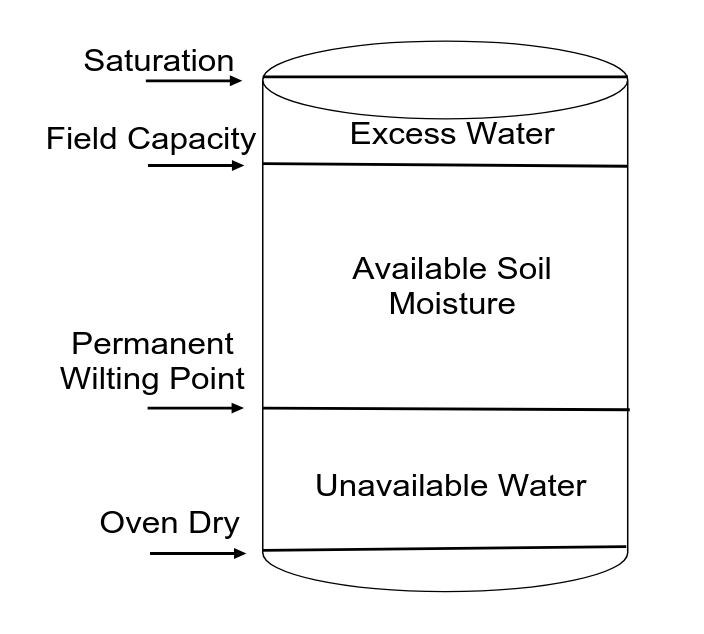
\includegraphics[width=0.5\linewidth]{./figures/SWC-costants.png}
    \caption{Valori soglia per \ac{SWC}\cite{Ding2022}.}
    \label{fig.SWC-costants}
\end{figure}

La quantità di acqua presente all'interno del terreno viene rappresentata dal \ac{SWC}, tipicamente misurato in percentuale di volume di acqua rispetto al volume del suolo.
In \cref{fig.SWC-costants}, è possibile vedere una serie di valori "soglia" che \ac{SWC} può raggiungere.\newline
Il termine \textit{saturation} indica uno stato in cui all'interno del terreno non è più presente l'aria e ogni poro è quindi pieno di acqua. Fatta eccezione per certi tipi di culture, come quella del riso, questo stato non è adatto alla crescita della pianta.\newline
Lo stato \textit{oven dry}, al contrario, avviene in totale assenza di acqua, non è quindi adatto alla crescita di nessun tipo di pianta.\newline
Viene definito \textit{\ac{FC}} il valore di \ac{SWC} massimo che permette alla pianta di assorbire l'acqua dal terreno. In questo stato i pori più grandi hanno al loro interno sia aria che acqua, mentre quelli più piccoli sono pieni di acqua.\newline
Infine, \textit{\ac{PWP}} è il punto dopo il quale la pianta non riesce più a estrarre acqua dal terreno, per quanto sia ancora in minima parte presente.\newline
Queste costanti, che sono meglio descritte in \cite{RAI2017505}, permettono di definire quale dovrebbe essere la percentuale di acqua nel suolo per permettere la crescita sana della piante: \ac{SWC} deve essere compreso tra \ac{FC} e \ac{PWP}.

Un ulteriore parametro è \ac{SWP}, potenziale idrico del suolo, rappresenta l'energia necessaria per estrarre l'acqua dal suolo e indica quindi la disponibilità di acqua delle piante. Viene espresso in termini di pressione e comprende diverse componenti che contribuiscono al valore finale\cite{MarshallT.J.TheoJohn1996Sp}. Le principali sono:

\begin{itemize}[noitemsep]
    \item \textbf{Potenziale gravitazionale}: deriva dalla forza di gravità e rappresenta l'energia potenziale dovuta alla sua posizione verticale.
    \item \textbf{Potenziale matriciale}: rappresenta l'energia necessaria per estrarre l'acqua dal suolo, risultante dalle forze d'interazione tra l'acqua e le particelle del suolo. È dovuto a forze come adesione e capillarità.
    \item \textbf{Potenziale osmotico}: rappresenta l'energia associata alla concentrazione di soluti e alla tendenza dell'acqua a muoversi da aree con alto potenziale osmotico (bassa concentrazione di soluti) ad aree con basso potenziale osmotico (alta concentrazione di soluti), come le radici delle piante.
\end{itemize}

La relazione tra \ac{SWP} e \ac{SWC} è definita dal concetto di \ac{SWRC}, curva di ritenzione idrica del suolo: la quantità di acqua trattenuta nel suolo a diversi livelli di pressione\cite{assouline1998water}.
\begin{figure}
    \centering
    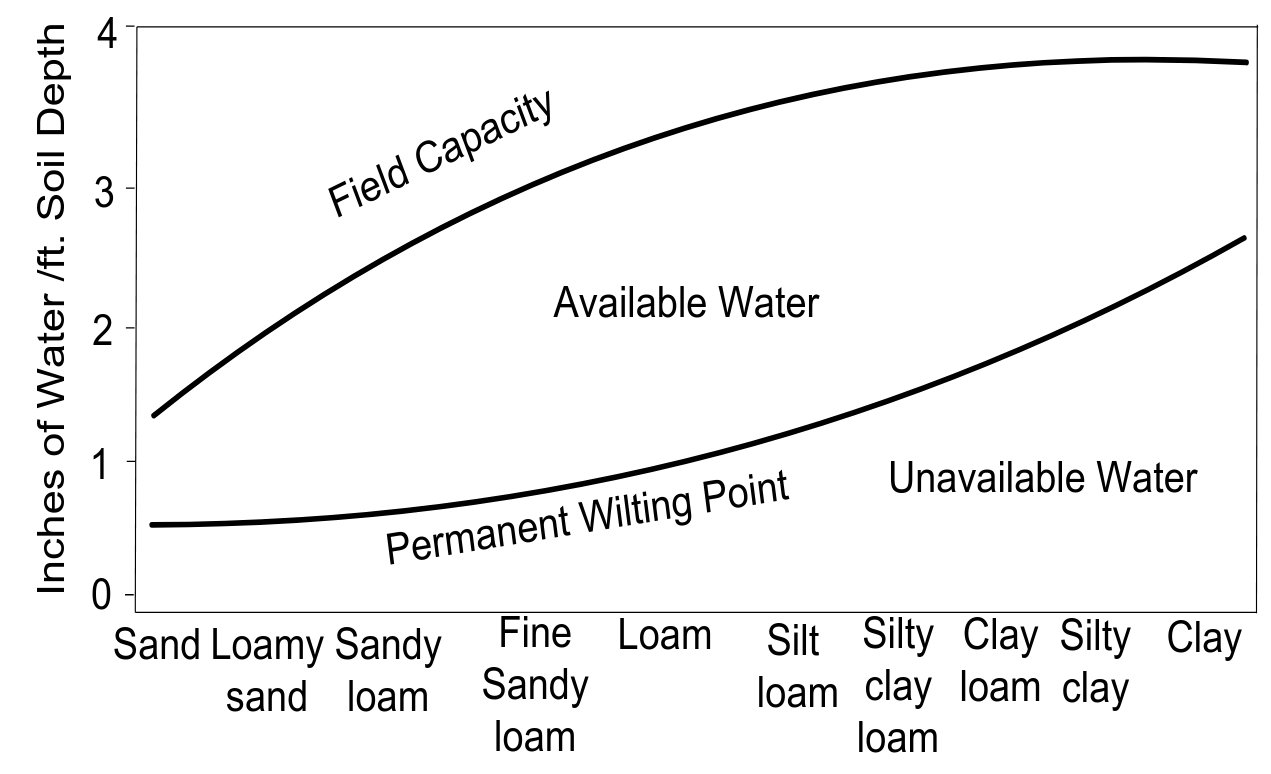
\includegraphics[width=0.5\linewidth]{./figures/SWC-costants-in-different-soils.png}
    \caption{Relazione tra le soglie e la tessitura del terreno\cite{Ding2022}.}
    \label{fig.SWC-costants-in-different-soils}
\end{figure}
\begin{figure}
    \centering
    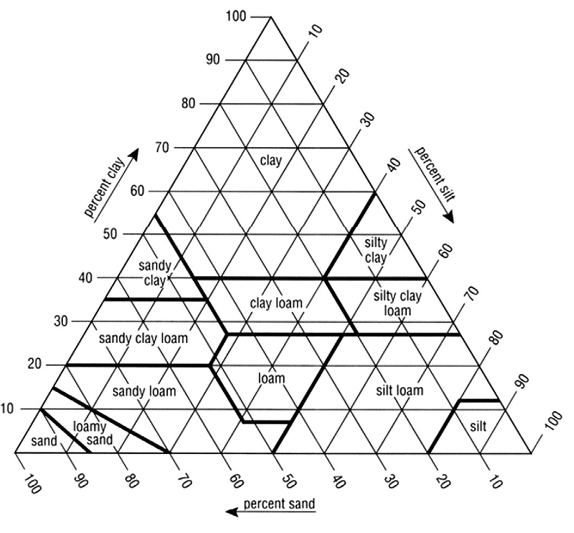
\includegraphics[width=0.8\linewidth]{./figures/soil-texture.png}
    \caption{Le classificazioni della distribuzione granulometrica del Dipartimento dell'Agricoltura degli Stati Uniti.\cite{RAI2017505}.}
    \label{fig.soil-texture}
\end{figure}
\begin{figure}[!tbp]
    \centering
    \begin{minipage}[t]{0.5\textwidth}
        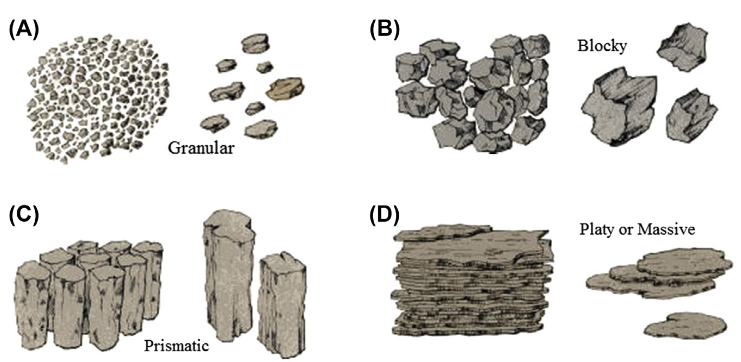
\includegraphics[width=\linewidth]{./figures/soil-structure.png}
        \caption{Classificazione del suolo in base alla struttura: (A) granulare, (B) a blocchi, (C) prismatico e (D) massiccio\cite{RAI2017505}.}
        \label{fig.soil-structure}
    \end{minipage}
    \hfill
    \begin{minipage}[t]{0.4\textwidth}
        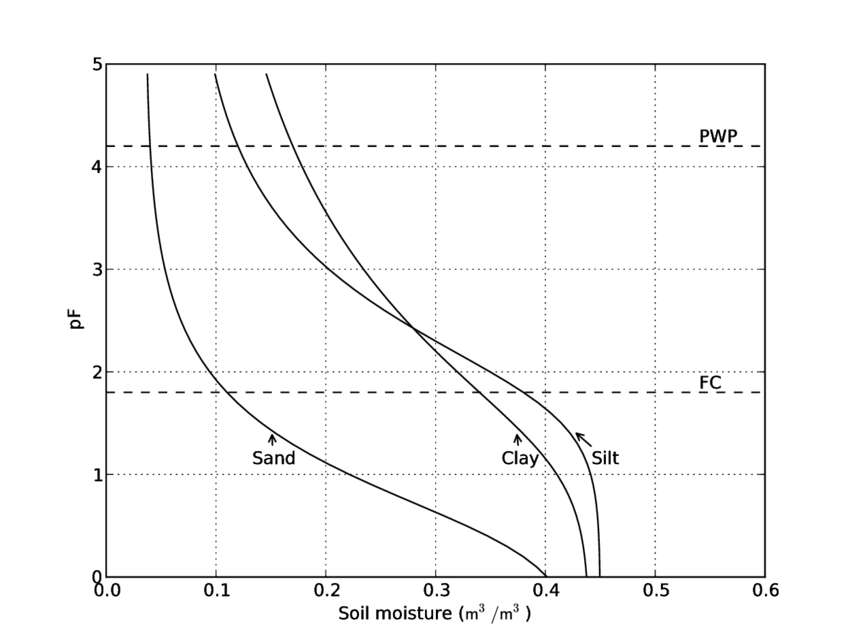
\includegraphics[width=\linewidth]{./figures/SWRC-In-different-soils.png}
        \caption{Curve di ritenzione idrica del suolo per tre diversi tipi di terreno. Le linee tratteggiate indicano la capacità di campo (FC) e il punto di appassimento permanente (PWP)\cite{Fuchsberger1023}.}
        \label{fig.SWRC-In-different-soils}
    \end{minipage}
\end{figure}
Tutti questi parametri dipendono da una serie di fattori, come:
\begin{itemize}[noitemsep]
    \item \textbf{Proprietà fisiche del terreno}, caratteristiche come la tessitura (distribuzione delle dimensioni delle particelle del suolo) e la struttura (raggruppamento in composti porosi delle particelle del suolo) hanno peso nella definizione di \ac{SWP}, e quindi chiaramente anche di \ac{SWRC}\cite{jury1990soil}. In \cref{fig.soil-texture} si possono vedere delle classificazioni comuni per i tipi di terreni in base alla tessitura, mentre in \cref{fig.soil-structure} in base alla struttura. In \cref{fig.SWRC-In-different-soils} sono presenti esempi di \ac{SWRC} per diversi tipi di terreno. Infine, in \cref{fig.SWC-costants-in-different-soils} è possibile vedere come i valori delle costanti precedentemente definite cambiano in base alla tessitura del terreno.
    \item \textbf{Coltura}, L'apparato radicale di una pianta ha effetto sul \ac{SWP} e quindi sulla \ac{SWRC}\cite{XIAO2024167524}.
\end{itemize}

È inoltre importante notare che sia l'apparato radicale che le proprietà fisiche del suolo non sono costanti all'interno dello stesso campo. A causa della quantità di variabili che possono modificare sostanzialmente la \ac{SWRC}, è molto difficile sapere di per certo la quantità d'irrigazione richiesta all'interno dell'intero campo senza monitorare attivamente l'andamento dell'acqua al suo interno.

Un ulteriore fattore da tenere in considerazione riguarda le variabili atmosferiche: di natura non modificabili, richiedono un monitoraggio continuo e preciso. Viene definita \textit{evapotraspirazione} il processo combinato attraverso il quale l'acqua viene trasferita nell'atmosfera, partendo da superfici d'acqua, dal ghiaccio, dal suolo e dalla vegetazione\cite{Kirkham2014}. Si tratta della combinazione tra \textit{evaporazione} e \textit{traspirazione}: la prima prevede il passaggio diretto dell'acqua nell'atmosfera e avviene per fattori come calore, umidità e velocità del vento; la seconda invece prevede il passaggio attraverso una pianta partendo dalle radici, fino a raggiungere le foglie, da dove avviene il passaggio all'atmosfera.
Le stazioni meteorologiche\cite{Allen1998CropE} sono in grado di monitorare, in un dato momento, il \textit{\ac{$ET_0$}}, evapotraspirazione potenziaole, che rappresenta il valore di evapotraspirazione in un dato momento di un ipotetica cultura di prato erboso in condizioni ottimali dove l'unico fattore limitante è dato dal clima, offre quindi una rappresentazione dell'acqua "perduta" e che non è più presente nel suolo. È possibile moltiplicare \ac{$ET_0$} per un \textit{\ac{$K_c$}}, coefficiente di coltura, che dipende dal tipo e dallo stato di crescita di una determinata cultura, per ottenere \ac{$ET_a$}: reale evapotraspirazione.
Questo permette quindi di approssimare la quantità di acqua usata da una pianta e che quindi deve essere somministrata tramite irrigazione, a patto che sia presente in letteratura una stima adeguata di $K_c$, che non è però sempre disponibile. Inoltre, \ac{$ET_0$} viene calcolato su un area potenzialmente molto estesa e potrebbe quindi non essere adeguato per campi con zone ombreggiate o venti locali.
% A ogni modo, il calcolo di \ac{$ET_a$} non tiene in considerazione le condizioni fisiche del suolo e dell'apparato radicale delle piante, per questo motivo il suo utilizzo esclusivo per decisioni riguardo l'irrigazione non è adeguato.

\subsection{Agricoltura di precisione}\label{agricoltura-precisione-tipi}

Vista la mole di variabili, diventa interessante utilizzare sistemi di monitoraggio e analisi col fine di consigliare gli agricoltori a come correttamente gestire i campi. Per questo nasce l'Agricoltura di Precisione: consiste nell'uso di tecnologie avanzate per aumentare l'efficienza, la produzione e la qualità dei prodotti\cite{ZHANG2002113}

Primi esempi di agricoltura di precisione, nel modo in cui viene intesa a oggi, risalgono già agli anni '80, dove lo sviluppo di modelli di crescita delle culture e l'utilizzo di \ac{GPS} ha permesso di mappare i campi e monitorare variabili spaziali come fertilità del suolo ed esigenze idriche\cite{201402720190101}.
Negli anni '90, l'introduzione di sensori per il monitoraggio delle variabili ha permesso agli agricoltori di adattare le loro pratiche in base alle esigenze specifiche di ciascuna area del campo\cite{201402720190101}.
Oggi l'arrivo di nuove tecnologie come Cloud Computing, \ac{IoT} e intelligenza artificiale ha portato un aumento sostanziale delle ricerche nel campo\cite{WOLFERT201769}.

Gli obbiettivi principali che si pone sono i seguenti:
\begin{itemize}[noitemsep]
    \item \textbf{Aumentare l'efficienza produttiva}: usando le risorse in modo più mirato si è in grado di ridurre gli sprechi.
    \item \textbf{Migliorare qualità e resa delle culture}: grazie al monitoraggio continuo è possibile rilevare rapidamente problemi come malattie, carenze nutrizionali o idriche potendo così intervenire tempestivamente.
    \item \textbf{Ridurre l'impatto ambientale}: ottimizzando l'utilizzo di risorse è possibile diminuire l'uso di acqua e di fertilizzanti, riducendo quindi l'impatto ambientale.
    \item \textbf{Supportare la sostenibilità economica}: l'input minore richiesto dagli agricoltori, insieme con l'uso inferiore delle risorse, ha anche un effetto positivo dal punto di vista economico. Oltre a rendere la cultura più resiliente a variazioni climatiche, diminuendo quindi costi di manutenzione in caso di eventi meteorologici estremi.
\end{itemize}

L'agricoltura di precisione si propone di agire in diverse aree dell'agricoltura, in base al contesto operativo, si può fare una divisioni nelle seguenti classi:
\begin{itemize}[noitemsep]
    \item \textbf{\ac{SSLM}}: un approccio all'agricoltura e alla gestione del territorio che adatta le decisioni e le pratiche alle caratteristiche uniche di specifiche aree all'interno di una fattoria o di un paesaggio. Invece di applicare tecniche uniformi su un intero campo o regione, la gestione sito-specifica utilizza informazioni dettagliate su suolo, clima, topografia e altri fattori ambientali per ottimizzare l'uso del terreno in ogni area. Si focalizza sull'ottimizzazione dell'uso del terreno \cite{SSLM}.
    \item \textbf{\ac{SSNM}}: si concentra sulla gestione mirata dei nutrienti necessari per le colture, come azoto, fosforo e potassio, adattandone l'applicazione alle condizioni specifiche di ogni parte del campo. L'obiettivo è migliorare l'efficienza d'uso dei fertilizzanti, riducendo gli sprechi e massimizzando la resa agricola, evitando allo stesso tempo danni ambientali legati all'eccesso di nutrienti \cite{SSNM}.
    \item \textbf{Precision Irrigation}: un sistema che ottimizza l'irrigazione fornendo la giusta quantità d'acqua in base alle necessità specifiche di ogni area del campo. Utilizzando dati su umidità del suolo, clima e tipologia di coltura, l'irrigazione di precisione permette di ridurre il consumo idrico e migliorare l'efficienza idrica, garantendo che le colture ricevano esattamente l'acqua necessaria per crescere in modo ottimale \cite{ANJUM202385}.
    \item \textbf{\ac{SSWM}}: un approccio che mira a gestire le infestanti in modo sito-specifico, applicando erbicidi o metodi di controllo solo nelle aree del campo dove le infestanti sono presenti o rappresentano una minaccia. Questo metodo riduce l'uso di prodotti chimici, minimizza l'impatto sull'ambiente e migliora l'efficacia delle pratiche di gestione delle infestanti \cite{SSWM}.
    \item \textbf{\ac{SSCP}}: si riferisce alla gestione delle malattie delle colture in modo sito-specifico, basandosi su dati raccolti riguardo alla distribuzione e gravità delle malattie in diverse parti del campo. Attraverso il monitoraggio e la diagnosi precoce, consente di applicare trattamenti solo nelle aree affette, riducendo l'uso di pesticidi e migliorando la salute complessiva del raccolto \cite{SSCP}.
\end{itemize}

\section{Componenti chiave dell’agricoltura di precisione}
\label{componenti-chiave}

Le tecnologie chiave dell'agricoltura di precisione sono tantissime, questo documento si limita a dare una panoramica generale.

\subsection{Acquisizione dati}

La raccolta dei dati è il fulcro dell'agricoltura di precisione: permettono di avere un'immagine reale delle condizioni dei campi, sia per quanto riguarda il suolo che a livello atmosferico.

\subsubsection{Remote Sensing}

Il Remote Sensing (\textit{telerilevamento}) è il processo di rilevamento e monitoraggio delle caratteristiche fisiche di un'area, misurando la radiazione riflessa ed emessa a distanza, tipicamente tramite satelliti o velivoli\cite{USGS-REMOTE-SENSING}.
L'analisi d'immagini ottiche e radar ad alta risoluzione, disponibili gratuitamente, viene utilizzata per monitorare i cambiamenti stagionali, la fenologia della vegetazione e le caratteristiche specifiche del territorio.
In ambito agricolo, il Remote Sensing è particolarmente utile per rilevare dati sulle coltivazioni, come lo stato di salute delle piante e l'umidità del suolo \cite{FAO-REMOTE-SENSING}. \newline
Il \ac{GPS}, sistema di posizionamento globale, è un sistema di navigazione satellitare che fornisce informazioni sulla posizione, la velocità e l'orario in tempo reale in qualsiasi parte del mondo \cite{GPS-GOV}.\newline
Il \ac{GIS}, sistema d'informazioni geografico, un sistema informativo che consente la raccolta, l'organizzazione, l'analisi e la visualizzazione di dati geografici. \newline
Integrando tecnologie come \ac{GPS} e \ac{GIS}, il Remote Sensing consente di creare mappe dettagliate che incorporano dati geo spaziali su vari aspetti di un territorio, come l'uso del suolo, la topografia, la distribuzione di risorse e le infrastrutture. Consente di sovrapporre diversi strati di dati e di analizzare le relazioni spaziali tra di essi attraverso mappe interattive. Il GIS può gestire grandi volumi di dati geografici, facilitando il monitoraggio e la pianificazione del territorio \cite{GIS-ESRI}.

\subsubsection{Sensori on-site}

Un ambito di ricerca molto attivo riguarda lo sviluppo di sensori in grado di monitorare le variabili delle coltivazioni, tenendo conto delle limitazioni legate all'uso in contesti agricoli: i campi estesi possono avere un accesso limitato a internet, e il consumo energetico deve essere ridotto a causa della scarsa disponibilità della rete elettrica, rendendo necessario l'uso di batterie, la cui durata deve essere massimizzata\cite{s24082647}.

Sono spesso utilizzate tecnologie di comunicazione wireless a lungo raggio, in particolare opzioni \ac{LPWA} come LoRa, NB-IoT e Sigfox, che sono emerse come alternative alle reti cellulari tradizionali (2G/3G/4G/5G)\cite{bhoyar2019communication}.
Le tecnologie LPWA sono caratterizzate da basso consumo energetico, bassa velocità di trasmissione dati, ampia copertura e supporto per connessioni massive. Le tecnologie LPWA eccellono nel collegare dispositivi che richiedono una trasmissione minima di dati su lunghe distanze con una lunga durata della batteria\cite{dai2019low}.

Aspetto fondamentale riguarda i sensori del suolo: sono in grado di misurare proprietà essenziali del suolo come il contenuto di umidità, la presenza e la quantità di nutrienti, la temperatura e il PH. Sono usati per orientare con precisione le pratiche d'irrigazione e fertilizzazione, evitando l'uso eccessivo di risorse e garantendo una disponibilità ottimale di nutrienti per le colture \cite{vuran2018internet}.

Sono inoltre disponibili sensori di qualità dell'acqua che sono in grando di monitorare aspetti come salinità, livelli di ossigeno disciolto e torbidità. Questi sensori svolgono un ruolo essenziale nel preservare l'idoneità dell'acqua d'irrigazione per la coltivazione e nel proteggere dal deterioramento del suolo causato da un eccesso di sali o contaminanti \cite{garcia2020iot}.

Alcuni sensori sofisticati sono in grado d'identificare l'esistenza di parassiti e malattie nelle colture. Utilizzano metodi come il riconoscimento delle immagini, la spettroscopia o altre tecniche per individuare la presenza di agenti patogeni o parassiti, consentendo un'azione rapida per mitigare i danni potenziali\cite{che2022mobile}.

Un componente fondamentale per l'acquisizione di dati in agricoltura di precisione è rappresentato dall'introduzione sul mercato di piattaforme hardware dotate di micro-controllori, come Arduino, ESP32 e altre soluzioni simili. Questi dispositivi sono in grado di ricevere i valori rilevati dai sensori distribuiti nei campi e di elaborare i dati raccolti, facilitando la gestione delle informazioni. Permettono di ridurre l'utilizzo di risorse e il costo del sistema, pur avendo un'elevata semplicità di programmazione. Possono essere programmati anche per attivare automaticamente sistemi d'irrigazione o allertare gli agricoltori su condizioni che richiedono interventi specifici\cite{iot4030012, su16010306}.

\subsubsection{Rilevazioni in laboratorio}

Le tecniche di misurazione in laboratorio possono essere utili per la raccolta di dati iniziali accurati e affidabili sulle caratteristiche del suolo. Tra le tecniche più comuni si trovano:
\begin{itemize}[noitemsep]
    \item Determinazione della densità apparente del suolo: prevede il prelievo di campioni di suolo mediante una trivella cilindrica, seguita dalla pesatura del campione umido e dall'essiccazione a 105°C per calcolare la densità apparente\cite{BULK-DENSITY}.
    \item Analisi della granulometria: consente di determinare la distribuzione delle dimensioni delle particelle del suolo, utilizzando metodi come la setacciatura e la sedimentazione. I risultati forniscono informazioni sulla capacità di ritenzione idrica e sull'aerazione del suolo\cite{GRANUMETRIC-ANALYSIS}.
    \item Determinazione del pH del suolo: il pH è un parametro cruciale che influisce sulla disponibilità dei nutrienti. La misurazione può essere effettuata in laboratorio mediante l'uso di un pH-metro su un campione di suolo mescolato con acqua distillata\cite{PH-SOIL}.
    \item Analisi della materia organica: la quantità di materia organica nel suolo è essenziale per la fertilità. Le tecniche di analisi includono l'uso di metodi chimici, come la combustione, per determinare il contenuto di carbonio organico\cite{ORGANIC-SOIL}.
    \item Test di capacità di ritenzione idrica: misura la quantità di acqua che un campione di suolo può trattenere dopo la saturazione. È fondamentale per comprendere la gestione dell'irrigazione e la sostenibilità delle colture\cite{WATER-RETENTION-LAB}.
\end{itemize}

In generale sono misurazioni che richiedono tempo, per questo motivo vengono effettuate saltuariamente.

\subsection{Simulazione del terreno}

I \ac{CSM}, modelli di simulazione delle colture, sono strumenti che simulano la crescita delle colture utilizzando equazioni biofisiche\cite{KELLY2023107986}.
Esistono diversi modelli \ac{CSM}, ognuno progettato per differenti casi d'uso.
Possono essere utilizzati per applicazioni di ricerca, per l'analisi di scenari o per la gestione delle colture. Nel ramo della ricerca vengono usati come strumento per aggregare le conoscenze o per integrare sperimentazioni sul campo, tipicamente molto costose. Un'altra applicazione dei modelli è quella di dimostrare l'impatto delle pratiche di gestione su una coltura o sull'ambiente agli agricoltori o ai responsabili politici\cite{MATTHEWS201324}.

I parametri dei modelli sono di solito determinati mediante la regolazione iterativa dei parametri e il confronto con i dati osservati dalle prove sul campo; Questo porta i valori stimati dei parametri ad essere imprecisi a causa degli errori sperimentali intrinseci associati all'osservazione sul campo. Un approccio usato negli ultimi anni per ovviare a queste imprecisioni riguarda la separazione dei i parametri del modello in fattori genetici così da creare modelli specifici per ogni cultura: gli autori di \cite{LI2012219} mostrano che questo approccio presenta diversi vantaggi rispetto ai metodi convenzionali.

\subsection{Software in supporto alle decisioni}

Un \ac{DSS}, sistema di supporto alle decisioni, è un sistema informativo in grado di supportare le attività decisionali fornendo raccomandazioni. Un \ac{DSS} efficace è un pacchetto software interattivo in grado di assistere agricoltori, consulenti o amministratori nel prendere decisioni che richiedono la sintesi di numerosi e diversi dati. In genere, i DSS incorporano uno o più modelli di simulazione che consentono di preparare raccomandazioni che tengono conto di fattori specifici della coltura e del luogo, come il clima, le date di semina, i tipi di terreno, le caratteristiche del sistema d'irrigazione.
I DSS sono generalmente pacchetti software che includono uno o più modelli di simulazione e strumenti di comunicazione per gestire gli input e gli output. Tra i sistemi per l'acquisizione dei dati, possono esserci collegamenti con servizi web specifici (ad esempio immagini satellitari, dati climatici in tempo reale, ecc.) e sensori che forniscono dati in tempo reale \cite{GALLARDO2020106209}.
\newpage

\section{Irrigazione di precisione}
\label{irrigazione-di-precisione}
% Definizione, breve related (presa dal paper in allegato), perchè è importante.

Questo documento ha interesse a mostrare un esempio di sistema d'irrigazione automatico su piccola scala, ricade quindi nella branca del Precision Irrigation, già definita in \cref{agricoltura-precisione-tipi}.

% Qua serebbe carino mettere le 5 caratteristiche che ha scritto il brother, solo che non voglio copia incollare, non posso citarlo essendo non pubblicato.

\subsection{Approcci di misurazione}\label{approcci-misurazione}

Tra i sensori descritti in \cref{componenti-chiave}, quelli che vengono utilizzati in questo contesto sono sia i sensori on-site che remoti.
I primi sono tipicamente posizionati sotto il terreno in modo da monitorare l'umidità del suolo, offrendo misurazioni precise.
I secondi invece vengono utilizzati per raccogliere valori a livello globale e sono di natura meno precisi.
In \cite{Babaeian2021} viene presentato un sistema che fa utilizzo di entrambe le tipologie di sensori, ma tipicamente è un approccio non utilizzato a causa dell'elevato costo.

I sistemi che fanno uso di sensori on-site possono essere classificati in base alla quantità di sensori posizionati per pianta. L'installazione più utilizzata, in quanto più economica, è quella a sensore singolo. Questa però pecca dell'impossibilità di monitorare l'umidità a diverse profondità\cite{Arif2013}.
I sistemi multi-sensore sono in grado di creare griglie multi-dimensionali.
La disposizione più utilizzata è quella di griglie mono-dimensionali, dove i sensori sono allineati verticalmente a diverse profondità sotto ad ogni pianta\cite{Karandish2016, Goldstein2017, Jimnez2020}.
Le griglie bidimensionali\cite{Egea2016, Cordeiro2016} prevedono l'installazione di più sensori per ogni strato, formando una matrice che descrive un'intera fetta di terreno. IMMAGINI
Le installazioni a griglia tridimensionale\cite{ZapataSierra2021, Liang2021}  possono essere viste come la visualizzazione di più fette di terreno.
Questi ultimi due tipi di installazione sono meno utilizzati a causa del maggior costo.

\subsection{Approcci all'irrigazione di precisione}

Contrariamente alla \cref{approcci-misurazione}, che si poneva l'obbiettivo di descrivere approcci alla misurazione, questa sezione ha come obbiettivo quello di descrivere alcuni approcci all'irrigazione: ogni approccio utilizza in modo diverso i dati raccolti nei diversi approcci di misurazione, con l'obbiettivo ultimo di somministrare la corretta quantità di acqua.

\subsubsection{Approcci classici}

L'approccio più semplice è rappresentato da sistemi basati su soglie, dove l'irrigazione viene fornita quando la misura dell'umidità del terreno è al di sotto di un determinato valore.
Questo genere di approcci soffre dell'inabilità di determinare il corretto volume di acqua necessaria al terreno, rendendoli adatti solo in ambienti controllati con poche variabili\cite{Zhao2023}.

Un altro approccio può essere trovato nell'utilizzo di della teoria dei controllori, progettati per gestire ambienti dinamici. Il loro utilizzo in campo aperto è scoraggiato dalla quantità di variabili incontrollabili.
Un esempio particolarmente importante riguarda l'utilizzo di controllori di tipo \ac{PID}, soluzione già ampiamente diffusa in altri ambiti\cite{Astrom1995}.
\cite{Goodchild2015} propone un sistema basato su un PID che permette di modellare, oltre all'umidità del terreno in input, le precipitazioni cadute. \cite{Lozoya2016} propone l'utilizzo di un \ac{MPC}, che secondo lo studio ha permesso un risparmio nel quantitativo di acqua utilizzato, mantenendo l'umidità all'interno di un intervallo ideale.

\subsubsection{Approcci basati sull'apprendimento autonomo}

Esistono approcci basati sull'apprendimento autonomo che sfruttando la diffusione dei dispositivi IoT per raccogliere grandi quantità di dati attraverso i quali addestrare modelli di machine learning: dalla classificazione\cite{Gloria2021}, alla regressione\cite{Navarro2016}, fino a sistemi più complessi che coinvolgono le reti neurali\cite{Gong2022} e il deep reinforcement learning\cite{Chen2021}.

Il problema principale in questo genere di approcci si trova nel rischio di over-fitting del modello: dati non sufficientemente eterogenei portano i modelli a essere addestrati per gestire culture specifiche, in uno stato di vita specifico, in specifiche condizioni del suolo e atmosferiche.
La raccolta di dati di alta qualità è quindi un processo costoso sia in termini economici che di tempo, soprattutto considerando che la raccolta dei dati è possibile solo durante le stagioni d'irrigazione.

In \cite{Gonzalez2019} è proposto un modello di predizione basato su reti neurali applicabile in contesti in cui la quantità di dati a disposizione è considerata limitata, ma la procedura di addestramento utilizza dati storici inerenti due anni solari di coltivazione, quantità superiore a quella spesso disponibile, si crea quindi un problema di cold-start: prima di avere un sistema di irrigazione in funzione, sono necessari due anni di misurazioni all'interno dei quali non è possibile utilizzare il modello.

Inoltre, gli autori di \cite{Silva2020} sottolinano la necessità di studi sul campo, evitando di basarsi esclusivamente ad ambienti simulati o controllati: i risultati derivati da tali ambienti spesso non sono trasferibili ad altri contesti oltre a quelli specificamente descritti negli studi.
Lo studio \cite{Alibaei2022} mostra un modello deep reinforcement learning applicato in un campo di pomodori in Portogallo, il cui obbiettivo è quello di massimizzare il guadagno rapportato alla quantità d'acqua utilizzata per la coltura.  Gli autori di \cite{García2020, Emmanuel2022} descrivono lo stato dell'arte in termini di sistemi di irrigazione intelligente.
Gli autori di \cite{Goldstein2017} confrontano tecniche di classificazione e di regressione mostrando che in ambi gli approcci i risultati sono stati corretti, rispetto alle scelte che avrebbe fatto un agronomo, con un accuratezza maggiore del 93\%. Gli autori di \cite{Sidhu2020} fanno riferimento solamente all'utilizzo di regressori, considerati più adatti visto il range continuo dell'output da determinare, portando a risultati con accuratezza del 71\% rispetto ad altri modelli, inoltre enfatizza l'importanza di una corretta modellazione e parametrizzazione del suolo. Gli autori di \cite{Emami2022} propongono un esempio di applicazione di un sistema di irrigazione intelligente su vasta scala utilizzando un Gaussian Process Regression Model.

Questo documento tiene in considerazione un sistema senza un suolo o cultura reale, per questo motivi approcci ad apprendimento autonomo non erano adeguati ed è stato preferito un approccio basato su un controllore \ac{PID}.

% \subsection{Algoritmo}

% \subsubsection{Approcci ideali}

% Si basano sull'idea che i fenomeni che fanno parte della crescita di una cultura siano deterministici.

% \paragraph{$ET_0$}

% Questo approccio fa puramente utilizzo di \ac{$ET_0$}. Il consiglio irriguo giornaliero è quindi la stima della quantità d'acqua perduta.

% \begin{equation}\label{irr}
%     \text{Irr}_q = ET_0
% \end{equation}

% I limiti di questo approccio, come visto in \cref{parametri-coltivazione}, è la natura di \ac{$ET_0$}, che porta con se approssimazioni intrinseche che possono risultare molto significative.

% \paragraph{Ottimo}

% Questo approccio utilizza l'idea dell'esistenza di uno stato "ottimo" del suolo, dove la quantità di acqua contenuta all'interno del terreno è ideale.
% Chiameremo $\text{WC}^*$ il \ac{SWC} ideale. Vogliamo quindi determinare per ogni stato attuale $WC_t$ il consiglio irriguo in modo che lo stato successivo $\text{WC}_{t+1}$ in cui si trova il terreno sia quello ottimo.

% \begin{flalign}
%     \text{WC}_{t+1} &= \text{WC}_t - ET_0 \label{wc-futuro} \\
%     \text{WC}^*     &= \text{WC}_t-ET_0+\text{Irr}_q\label{wc-ottimo} \\
%     \text{Irr}_q    &= \text{WC}^*-\text{WC}_t+ET_0\label{irr-con-ottimo}
% \end{flalign}

% In un contesto in cui il sistema in esame è deterministico e accurato, è possibile esprimere relazioni esatte tra i fenomeni in atto, come vediamo in \cref{wc-futuro}.
% È possibile definire lo stato del giorno successivo assumendo l'assenza di precipitazioni e che il valore di evapotraspirazione potenziale sia effettivamente rappresentativo della quantità di acqua persa da un terreno in un giorno.
% Come definito in \cref{wc-ottimo}, lo scopo della procedura d'irrigazione è fare in modo che il \ac{SWC} del giorno successivo sia quello ottimo. È quindi possibile, dato lo stato attuale e uno ottimo, definire il consiglio irriguo, come in \cref{irr-con-ottimo}

% \subsubsection{Approcci ponderati}

% Questi approcci cercando di modellare le approssimazioni introdotte dalla parametrizzazione dei fenomeni analizzati.

% \paragraph{Delta}\label{delta}

% Questa soluzione vuole modellare l'errore commesso nella stima di \ac{$ET_0$}.

% \begin{equation}\label{irr-delta}
%     \text{Irr}_q = ET_0 \pm \delta
% \end{equation}

% Utilizza quindi \cref{irr} ma pondera un'azione correttiva $\delta$, il cui valore viene aggiornato prima di ogni irrigazione. Sia $r$ la differenza tra lo stato del suolo al tempo $t$ e lo stato del suolo "ottimo"; Siano $\gamma$ e $\varepsilon$ rispettivamente il parametro correttivo che determina $r$ e la tolleranza accettata per $r$

% \begin{empheq}[left={\delta_t=\empheqlbrace}]{align}
%     \delta_{t-1} & && \hspace*{-8em} \text{se } -\varepsilon < r < \varepsilon \label{pond-1}\\
%     \delta_{t-1} & + \gamma && \hspace*{-8em} \text{se } r < -\varepsilon \label{pond-2} \\
%     \delta_{t-1} & - \gamma && \hspace*{-8em} \text{se } r > \varepsilon \label{pond-3}
% \end{empheq}

% A ogni determinazione del consiglio irriguo, se la differenza tra lo stato attuale e quello ottimo è all'interno di un range di tolleranza (\cref{pond-1}) il valore di $\delta_t$ rimane costante. Se il suolo è più asciutto del caso ottimo (\cref{pond-2}) allora il valore di $\delta_t$ viene aumentato di $\gamma$.  Al contrario, se il terreno è troppo bagnato, il valore di $\delta_t$ viene diminuito di $\gamma$(\cref{pond-3}).

% Se suddividiamo il terreno in celle di cui possiamo misurare la percentuale di acqua, possiamo definire con alta granularità la differenza tra lo stato ottimo $\text{WC}^*$ e lo stato attuale $\text{WC}_t$ come la differenza cella per cella.

% \begin{equation}\label{r}
%     r = \frac{\sum\limits_{i=0}^h \sum\limits_{j=0}^w (WC_{t[i,j]} - WC^*_{[i,j]})}{h \times w}
% \end{equation}

% Dove $h$ e $w$ sono rispettivamente righe e colonne delle matrici del suolo.

% \paragraph{Matrice di costo}

% L'approccio visto in \cref{delta} non tiene in considerazione come esattamente sia distribuita l'acqua all'interno del suolo, che come abbiamo visto non è necessariamente distribuito allo stesso modo in tutto il terreno. In questo modo, due terreni con distribuzione totalmente diversa ma la cui media di potenziale idrici produceranno lo stesso consiglio irriguo.
% Questo è un problema in quanto celle con maggiore densità radicale necessitano una quantità d'acqua maggiore rispetto a celle con bassa densità radicale. \note{dire da qualche parte sta cosa}
% Avere un modo di calcolare il consiglio irriguo in base alla distribuzione d'acqua nel terreno porterebbe quindi a un risparmio d'acqua, permettendo di fornire l'irrigazione necessaria in base alla densità radicale.

% Sfruttando la natura cella per cella del calcolo di $r$ secondo l'\cref{r} è possibile associare a ogni cella di $\text{WC}_t$ un valore nell'intervallo [0,1] che ne rappresenti l'importanza nella fetta di suolo in esame.

% \begin{equation}\label{r-matrice-costo}
%     r = \frac{\sum\limits_{i=0}^h \sum\limits_{j=0}^w (WC_{t[i,j]} - WC^*_{[i,j]})\times C_{[i,j]}}{h \times w}
% \end{equation}

% \section{Limitazioni attuali dell’agricoltura di precisione}
% \label{limiti}
% Costi e accessibilità per i piccoli agricoltori
% Sfide legate alla raccolta e gestione dei dati

% RIGUARDA LA FREQUENZA; DA CITARE DOPO Il problema nella determinazione del consiglio irriguo è rappresentato dalla determinazione della frequenza e quantità (Irrq) d’acqua con cui irrigare. In letteratura è possibile trovare esempi che considerano frequenze d’irrigazione diverse: oltre ai più comuni approcci a frequenza giornaliera [27, 78, 80] gli autori di [83] propongono un modello per il calcolo di un consiglio irriguo della durata di quattro giorni mentre [43] modella il problema con granularità settimanale; questo lavoro considera un modello ad irrigazione giornaliera.

% \chapter{Tecnologie utilizzate}


% %Descrive appunto le tecnologie utilizzate nel progetto: sia lato HW (Arduino + Raspberry + sensori), sia lato SW (stack tecnologico). Lunghezza 5-8 pagine.


% \section{Hardware}

% \begin{itemize}[noitemsep]
%     \item \textbf{Sensori}, TODO numero sensore e citazione alle specifiche
%     \item \textbf{Arduino UNO R3} è una scheda microcontrollore basata sull'ATmega328P. Permette di caricare i programmi scritti in linguaggio C++ usando un'architettura SuperLoop, dove un unico pezzo di codice viene ripetuto fin tanto che il dispositivo è riceve alimentazione. Il superloop è interrompibile momentaneamente solo tramite degli interrupt di sistema, che vengono gestiti con routine non interrompibili, ciò implica che durante una routine, non possono avvenire altri interrupt. È quindi consigliabile che le routine di gestione siano particolarmente brevi, sia per evitare perdita di eventi, sia perchè molte librerie di sistema sfruttano internamente gli interrupt, per esempio \texttt{delay} (equivalmente a sleep di python). Offre l'utilizzo di un totale di 22 pin \ac{GPIO}: 16 dei quali digitali, di cui 6 utilizzabili come output analogici tramite \ac{PWM}, e altri 6 pin input analogico. Può inoltre gestire una comunicazione seriale tramite USB con la quale è possibile comunicare con altri dispositivi.
%     \item \textbf{Raspberry Pi 4 model B} è un \ac{SBC} in grado di utilizzare sistemi operativi veri e propri basati sul kernel Linux o su RISC OS. Presenta un processore quad-core ARM a 64bit ad una velocità di clock di 1.80GHz. La configurazione utilizzata presenta \note{QUANTITARAM} Gb di RAM LPDDR4-3200. Compatibile con Bluetooth 5.0, BLE, connessioni wireless IEEE 802.11ac a 2.4 GHz e 5.0 GHz, oltre che Gigabit Ethernet. Permette anche l'utilizzo di 40 pin GPIO digitali. Compatibile con periferiche USB tramite 2 porte USB2.0 e 2 porte USB3.0. L'uscita video è permessa da tramite 2 porte Micro-HDMI, che supportano dual-screen 4k. Come storage viene utilizzata una singola scheda microSD. Include un'interfaccia MIPI DSI per display e MIPI CSI per telecamere, ed è alimentato tramite un connettore USB-C da 5V/3A. Prodotto dalla Raspberry Pi Foundation, che ha realizzato diversi modelli per varie esigenze, è compatibile con vari sistemi operativi, tra cui il più noto è Raspberry Pi OS (precedentemente chiamato Raspbian), una versione di Debian sviluppata dalla stessa fondazione.
% \end{itemize}

% \section{Software}

%     \begin{itemize}[noitemsep]
%         \item \textbf{\ac{JS}} è un linguaggio di programmazione interpretato, usato principalmente per la programmazione web sia a livello client che server, per esempio con l'utilizzo di Node.js. È un linguaggio dinamico, basato sui prototipi, multi-paradigma, single-threaded , che supporta stili di programmazione orientati agli oggetti, imperativi e dichiarativi. Standardizzato come ECMAScript, \ac{JS} è alla base di un vasto ecosistema di librerie e framework che ne ampliano le capacità e l'applicabilità in diversi contesti.
%         \begin{itemize}[noitemsep]
%             \item \textbf{Chart.js} è una libreria \ac{JS} semplice e flessibile per la generazione di grafici lato frontend. Si tratta di un progetto Open Source che sfrutta i canvas di HTML5. Di default permette l'utilizzo di 8 diversi tipi di grafici, è compatibile con plug-in che permettono l'aggiunta di nuove funzionalità.
%             \begin{itemize}[noitemsep]
%                 \item \textbf{chartjs-chart-matrix} è un plug-in che permette la creazione di grafici a matrice, un esempio è in \cref{fig.matrix_chart_example}
%                 \begin{figure}
%                     \centering
%                     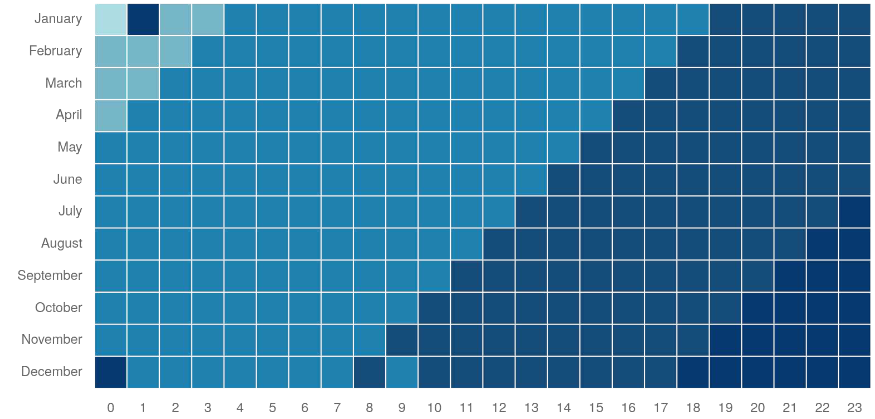
\includegraphics[width=0.9\linewidth]{./figures/matrix-chart-example.png}
%                     \caption{Esempio di una mappa delle temperature medie giornaliene per mese, l'intensità del colore è proporzionale alla temperatura.}
%                     \label{fig.matrix_chart_example}
%                 \end{figure}
%                 \item \textbf{chartjs-plugin-streaming} è un plug-in che permette la creazione di grafici con valori in tempo reale. Prevede lo scorrimento verso sinistra del grafico in base al tempo. È possibile configurarlo per moficare la granularità, la frequenza di aggiornamento ed un eventuale delay in modo da avere una visualizzazione "fluida" dei nuovi dati. Necessita di un adapter per una libreria per la gestione delle date e ricezione del tempo attuale, come Luxon.
%                 \item \textbf{chartjs-plugin-datalabels} è un plug-in per la visualizzazione dei dati su un grafico, un esempio su un grafico a linea è visibile in \cref{fig.datalabels-example}
%                 \begin{figure}
%                     \centering
%                     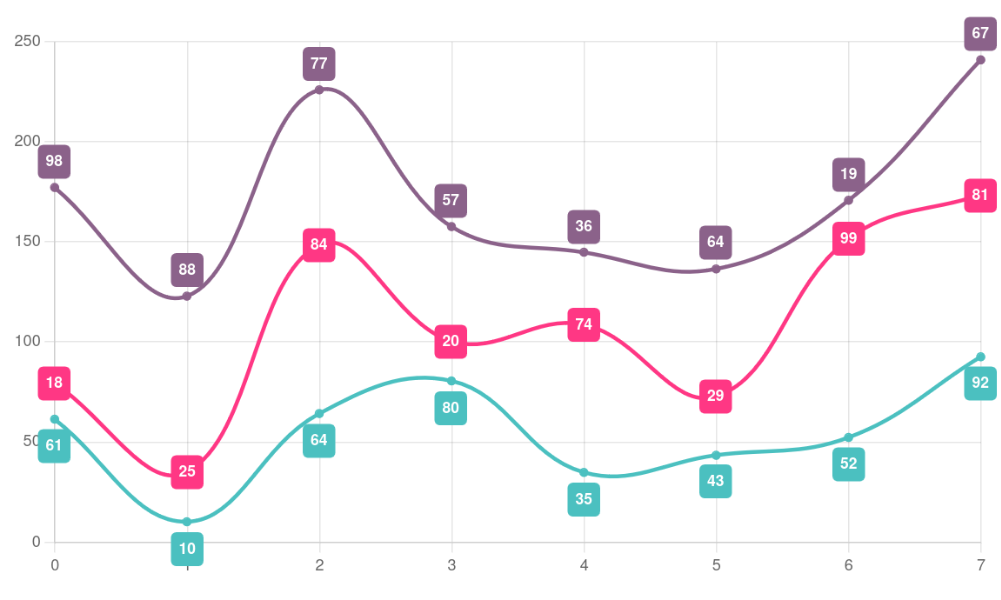
\includegraphics[width=0.9\linewidth]{./figures/datalabels-example.png}
%                     \caption{Esempio utilizzo di datalabels dove in ogni linea la posizione del label è differente.}
%                     \label{fig.datalabels-example}
%                 \end{figure}
%                 \item \textbf{chartjs-adapter-luxon} è un plug-in che si occupa di fornire a chartjs-plugin-streaming le informazioni sulle date da Luxon.
%             \end{itemize}
%             \item \textbf{Luxon} è un wrapper di date e tempi per \ac{JS}. Utilizza un'API per gestiore le date, che consente il supporto agli intervalli, alle durate (14 days, 5 minutes, 33 seconds), la loror conversione e parsing. Offre la localizzazione delle stringhe con una gestione interna delle time-zones.
%             \item \textbf{bootstrap} è un toolkit frontend potente ed estendibile. Permette la creazione di interfacce web utilizzando unicamente classi HTML, senza la necessità di scrivere il proprio foglio di stile CSS.
%             \item \textbf{jQuery} è una famosa libreria per la manipolazione e navigazione di documenti HTML, la gestione degli eventi, le animazioni e richieste HTTP.
%             \item \textbf{Socket.io} permette l'apertura di una comunicazione bidirezionale sempre attiva tra client e server utilizzando WebSocket.
%         \end{itemize}
%         \item \textbf{Python} è un linguaggio di programmazione ad alto livello che supporta il paradigma object-oriented, la programmazione struttrata e molte caratteristiche di programmazione funzionale. È un linguaggio debolmente tipizzato, che utilizza unicamente l'indentazione per la definizione dei blocchi di codice, al contrario di molti linguaggi, non prevede quindi l'utilizzo di parentesti graffe. Supporta l'overloading di operatori e funzioni tramite delegati, oltre che sinstassi avanzate quali slicing (l'utilizzo di un certo range di elementi in una lista) e list comprehension (la creazione di nuove liste partendo da una originale). Il codice python viene interpretato (con delle compilazioni a bytecode alla prima esecuzione per migliorare le performance) che supporta anche un uso interattivo.
%         \begin{itemize}[noitemsep]
%             \item \textbf{Flask} è un framework web per la creazione di backend per Python.
%             \item \textbf{Flask-SocketIO} è una libreria Python per la gestione di websocket tramite Socket.io.
%             \item \textbf{NumPy} è la libreria principale per il calcolo scientifico Python. Permette la gestione di array $n$-dimensionali ed è ampiamente utilizzato per operazioni di algebra lineare, trasformate di Fourier, manipolazioni di dati e altre applicazioni numeriche. È uno strumento essenziale per chi lavora con analisi numeriche, machine learning e data science.
%             \item \textbf{pySerial} è una libreria per l'accesso a porte seriali. Permette la stessa gestione delle porte seriali su ogni piattaforma. Supporta diversi byte size, bit di parità e di fine messaggio, oltre che controllo del flusso. La porta è configurata per la trasmissione binaria.
%             \item \textbf{dotenv} è un modulo per la gestione delle variabili d'ambiente.
%             \item \textbf{pytz} è una libreria per il calcolo del fuso orario in python.
%             \item \textbf{SciPy} è una libreria di Python per il calcolo scientifico e tecnicho, espande NumPy. Offre un'ampia quantità di funzionalità per l'ottimizzazione, la statistica, l'integrazione, l'algebra lineare, l'elaborazone dei segnali, la gestione di immagini e altre operazioni matematiche avanzate. È molto utilizzata per esempio nei campi della fisica, dell'ingegneria, della biologia computazionale.
%         \end{itemize}
%         \item \textbf{C++} è un linguaggio di programmazione nato come espansione del linguaggio C, presenta caratteristiche di programmazione funzionale, generica e orientata agli oggetti, permettendo però una gestione a basso livello della memoria. Per quest'ultima caratteristica è tipicamente utilizzato in contesti dove le prestazioni sono particolamente importanti come lo sviluppo di sistemi operativi, software embedded, motori di gioco e applicazioni real-time. In particolar modo è utilizzanto anche per lo sviluppo di software per dispositivi con risorse limitate, come microcontrollori e sistemi embedded, dove la gestione diretta della memoria e delle risorse hardware è essenziale.
%         \begin{itemize}[noitemsep]
%             \item \textbf{Arduino API} è una libreria in C/C++ per la scrittura di codice per dispositivi Arduino. Contiene funzioni riguardanti l'hardware, per esempio, contiene funzioni per la lettura/scrittura di segnali digitali e analogici sui pin, per la gestione degli interrupt e della porta seriale. Oltre alle funzioni hardware, l'API include, ad esempio, strumenti per la gestione dei timer, funzioni matematiche, funzioni per la gestione di bit e byte e per la gestione degli stream. Contiene inoltre i tipi di variabile `enum`, `String` e funzioni per la conversione.
%             \item \textbf{TimerInterrupt} è una libreria che permette l'utilizzo del timer fisico di una board Arduino come interrupt di sistema, permettendo lo svolgimento ininterrotto di ruotine periodicamente.
%             \item \textbf{ArduinoJson} è una semplice libreria per la gestione di stringhe JSON su piattaforma Arduino. Permette serializzazione e deserializzazione, ed è quindi molto utile per mandare dati strutturati sul seriale in modo che venga che lo scambio dei dati sia standardizzato.
%         \end{itemize}
%     \end{itemize}



% \chapter{Un prototipo di irrigazione prescrittivo}
% Descrive nel dettaglio il tuo lavoro, quindi come le tecnologie presentate nella precedente sezione sono state utilizzate nel progetto. Puoi prenderla larga descrivendo il nostro sistema (quello che ti ho mostrato sul mio pc) per poi descrivere la necessità di averne una rappresentazione su piccola scala e come è stata realizzata, così come descrivere il ciclo di vita del dato (collection, processing, exploitation). Ora come ora è normale tu non abbia chiare le idee su questo capitolo, andando avanti integreremo le tue conoscenze con quelle pregresse nostre sul dominio applicativo e sul nostro sistema. Questo capitolo deve essere il core della tesi, lunghezza 20 pagine.

% \chapter{Conclusioni e sviluppi futuri}

% Breve capitolo che trae le conclusioni sul lavoro svolto, il risultato ottenuto rispetto a quello atteso e lo spazio dedicato a migliorie future.

%
% BIBLIOGRAPHY
%

\backmatter

\bibliographystyle{unsrt}
\bibliography{bibliography}

\begin{acknowledgements} % this is optional
    Optional. Max 1 page.
\end{acknowledgements}

\end{document}
